\section[质心定理]{\makebox[5em][s]{质心定理}}\label{sec:08.04}

本节讨论动量守恒的另一种描述方式。

我们首先讨论由质量为$ m _ { 1 } , m _ { 2 } $,位置矢量
为$ \vec { r } _ { 1 } , \vec { r } _ { 2 } $的两个质
点所构成的孤立体系(图\ref{fig:08.09})这个体系的动量守恒,即
\begin{equation*}
  \frac { \dif \vec { P } } { \dif t } = 0
\end{equation*}
或\vspace{-0.5em}
\begin{equation}\label{eqn:08.04.01}
  \begin{split}
    \vec { P } & = m _ { 1 } v _ { 1 } + m _ { 2 } v _ { 2 } \\
    & = m _ { 1 } \frac { \dif \vec { r } _ { 1 } } { \dif t } + m _ { 2 } \frac { \dif \vec { r } _ { 2 } } { \dif t } \\
    & = \frac { \dif } { \dif t } \left( m _ { 1 } \vec { r } _ { 1 } + m _ { 2 } \vec { r } _ { 2 } \right) \\
    & = \left( m _ { 1 } + m _ { 2 } \right) \frac { \dif } { \dif t } \left( \frac { m _ { 1 } \vec { r } _ { 1 } + m _ { 2 } \vec { r } _ { 2 } } { m _ { 1 } + m _ { 2 } } \right) \\
    & = \left( m _ { 1 } + m _ { 2 } \right) \frac { \dif \vec { r } _ { c } } { \dif t } \\
    & = \text { 不变量 }
  \end{split}
\end{equation}
其中,我们用了一个新的物理量$ \vec { r } _ { c } $,定义为
\begin{equation}\label{eqn:08.04.02}
  \vec { r } _ { c } \equiv \frac { m _ { 1 } \vec { r } _ { 1 } + m _ { 2 } \vec { r } _ { 2 } } { m _ { 1 } + m _ { 2 } }
\end{equation}
它表示一个位置,即图8.7中的$ C $点,称为体系的质心位置。

对式\eqref{eqn:08.04.01}再次求导,得
\begin{equation*}
  \left( m _ { 1 } + m _ { 2 } \right) \frac { \dif ^ { 2 } \vec { r } _ { c } } { \dif t ^ { 2 } } = 0
\end{equation*}
\begin{align}\label{eqn:08.04.03}
  \beforetext{即} \frac { \dif ^ { 2 } \vec { r } _ { c } } { \dif t ^ { 2 } } = 0
\end{align}
式\eqref{eqn:08.04.03}表明,对孤立体系,其质心的加速度为零,即$ C $点的加

% 240.jpg
\begin{wrapfigure}[10]{r}{13em}
  \centering
  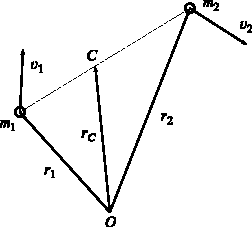
\includegraphics{figure/fig08.09}
  \caption{质心}
  \label{fig:08.09}
\end{wrapfigure}
\noindent 速度为零。因此,动量守恒定律又可陈述为:孤立体系的质心作
匀速直线运动或静止,这就是质心定理。

应当强调,质心可能并不在体系中的任何一个质点上,它是
由式\eqref{eqn:08.04.02}形式定义的一个物
理量。这里我们第一次看到,一个有用的物理量,可能并不对应
着一个实际的东西。这种具有抽
象性质的物理量,在以后的物理学中,我们将会越来越多地碰
到。

很容易把质心定理推广到多质点构成的孤立体系。由动量守
恒定律,用上述类似的推导可知,一个由
$ m _ { 1 } , m _ { 2 } , \cdots , m _ { n } $
质点所构成伪体系,其质心位置应是
\begin{equation}\label{eqn:08.04.04}
  \vec { r } _ { c } = \frac { m _ { 1 } \vec { r } _ { 1 } + m _ { 2 } \vec { r } _ { 2 } + \cdots + m _ { n } \vec { r } _ { n } } { m _ { 1 } + m _ { 2 } + \cdots + m _ { n } }
\end{equation}
其中$ \vec { r } _ { 1 } , \vec { r } _ { 2 } , \cdots , \vec { r } _ { n }$分别为各质点的位置。
这时,动量守恒定律可写为\vspace{-0.4em}
\begin{equation}\label{eqn:08.04.05}
  \frac { \dif ^ { 2 } \vec { r } _ { c } } { \dif t ^ { 2 } } = 0
\end{equation}

现在我们进一步讨论不仅有内力作用,而且也有外力作用的
非孤立体系的情况。我们仍采取上述质心的定义,则质心速度为
\begin{equation*}
  \begin{split}
    \vec { v } _ { c } & = \frac { \dif \vec { r } _ { c } } { \dif t } \\
    & = \frac { 1 } { \sum \limits _ { i = 1 } ^ { n } m _ { i } } \left( m _ { 1 } \frac { \dif \vec { r } _ { 1 } } { \dif t } + m _ { 2 } \frac { \dif \vec { r } _ { 2 } } { \dif t } + \cdots + m _ { n } \frac { \dif \vec { r } _ { n } } { \dif t } \right) \\
    &= \frac { 1 } { \sum \limits _ { i = 1 } ^ { n } m _ { i } } \left( m _ { 1 } \vec { v } _ { 1 } + m _ { 2 } \vec { v } _ { 2 } + \cdots + m _ { n } \vec { v } _ { n } \right)
  \end{split}
\end{equation*}
质心的加速度为
\begin{equation}\label{eqn:08.04.06}
  \begin{split}
    \frac { \dif \vec { r } } { \dif t } & = \frac { 1 } { \sum \limits _ { i = 1 } ^ { n } m _ { i } } \left( m _ { 1 } \frac { \dif \vec { v } _ { 1 } } { \dif t } + m _ { 2 } \frac { \dif \vec { v } _ { 2 } } { \dif t } + \cdots + m _ { n } \frac { \dif \vec { v } _ { n } } { \dif t } \right) \\
    & = \frac { 1 } { \sum \limits _ { i = 1 } ^ { n } m _ { i } } \left( \vec { F } _ { 1 } + \vec { F } _ { 2 } + \cdots + \vec { F } _ { n } \right)
  \end{split}
\end{equation}
其中$ \vec { F } _ { i } $是第$ i $个质点所受到的总力,等于内力与外力之和。

根据牛顿第三定律,体系的内力成对出现,且大小相等,方
向相反,所以在式\eqref{eqn:08.04.06}中内力全部相互抵消了。
因此\eqref{eqn:08.04.06}式成为
\begin{equation*}
  \frac { \dif \vec { r } _ { c } } { \dif t } = \frac { 1 } { \sum \limits _ { i = 1 } ^ { n } m _ { i } } \left( \vec { F } _ { 1 \text {外} } + \vec { F } _ { 2 \text {外} } + \cdots + \vec { F } _ { n \text {外} } \right)
\end{equation*}
或
\begin{equation}\label{eqn:08.04.07}
  M _ { \text {总} } \frac { \dif \vec { v } _ { c } } { \dif t } = \vec { F } _ { \text {外} }
\end{equation}
其中$ M _ { \text {总} } = \sum\limits _ { i = 1 } ^ { n } m _ { i } $,
称为体系的总质量;
$ \vec { F } _ { 1 \text {外} } + \vec { F } _ { 2 \text {外} } + \cdots + \vec { F } _ { n \text {外} } $
是体系所受到的总外力;$ \vec { F } _ { i \text {外} } $
是第$ i $个质点所受外力。

式\eqref{eqn:08.04.07}就是质心定理的一般形式,它是非常有用的。
我们知道,一个体系的运动,一般是相当复杂的,因为$ n $个质点都
在相互运动,不仅有内力,还要考虑外力。但是,
式\eqref{eqn:08.04.07}告诉我
们,如果不考虑每个质点运动的细节,而只考虑体系的质心运动,
则其动力学方程与单个质点的动力学方程完全相同。这就是说,
一个体系,在某些方面可用一个质点来标志,这个质点的质量等
% 242.jpg
于体系的总质量,位置在质心,所受的力等于体系的外力的总
和,它的运动满足牛顿第二定律。不管内力如何复杂,这个结论
是普遍适用的。我们常把很大的物体(譬如地球)看为质点,其根
据正在于此。在考虑地球的某些方面的运动,譬如说绕太阳的整
体运动,可以把它作为质点来处理。虽然地球内部有各种各样的
互作用,却可以完全不必顾及,只需考虑外力——太阳引力的
作用就行了。

应当再强调一点,在式\eqref{eqn:08.04.07}中,总质量
$ M _ { \text {总} } $是各质点质量之和,即
\begin{equation}\label{eqn:08.04.08}
  M _ { \text {总} } = m _ { 1 } + m _ { 2 } + \cdots + m _ { n }
\end{equation}
这个等式似乎很平凡,谁都知道,复杂物体的质量等于各部分的
质量之和。但若仔细考察这个关系,也并不那么显然。宏观物体
都是由分子、原子构成的,而原子、分子在不停的运动着,为什
么物体的总质量与分子及原子的复杂运动状态无关,而一定等于
各分子、原子的质量之和呢?这并不是显而易见的。因此,我们
应当记住,式\eqref{eqn:08.04.08}只是牛顿力学中的一个
结果,而并不是不证自明的。
